\documentclass[10pt,a4paper]{article}
\usepackage[utf8]{inputenc}
\usepackage[german]{babel}
\usepackage{amsmath}
\usepackage{amsfonts}
\usepackage{amssymb}
\usepackage{graphicx}
\usepackage[top=1cm,bottom=1cm]{geometry}

\begin{document}
	
\pagestyle{empty}
		\begin{center} 
			
\includegraphics[scale=0.3]{./Dateien/UniKoelnLogo.jpeg}
			\vspace*{2cm} 
			
			
			\large 
			Bachelorarbeit
			\vspace*{1cm}
			
			{\huge \textbf{Der Endlichkeitssatz für $H^1(X,\mathcal{O})$ auf \\[0.5cm]kompakten Riemannschen Flächen}}
			\vspace*{1cm}
			
			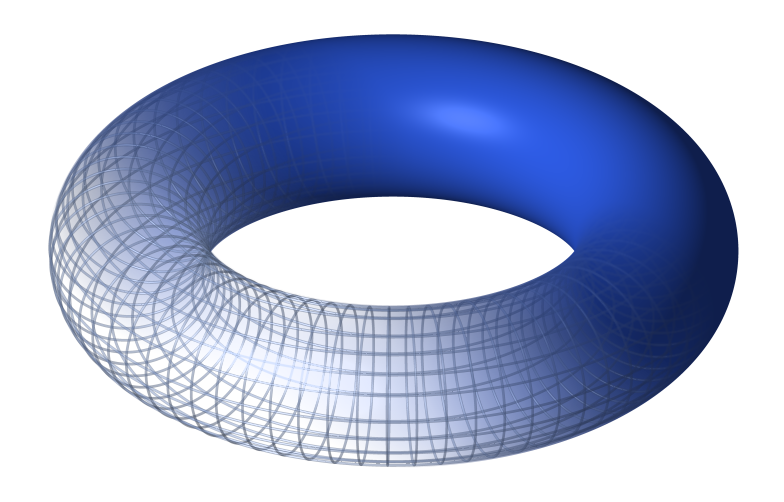
\includegraphics[scale=0.2
			]{./Dateien/Torus.png}
			\vspace{1.5cm}
			
			Aurelio Marafioti
			
			7306409
			\vspace*{1cm}
			
			\today
			\vspace*{1.5cm}
			
			\small{
			Betreuung: Prof. Dr. George Marinescu \\
			Mathematisches Institut \\
			Universität zu Köln}
		\end{center}

\end{document}